\section{Bilag}

\subsection{DCD}
\begin{figure}[H]
    \caption{Relation for vores DCD}
    \centering
        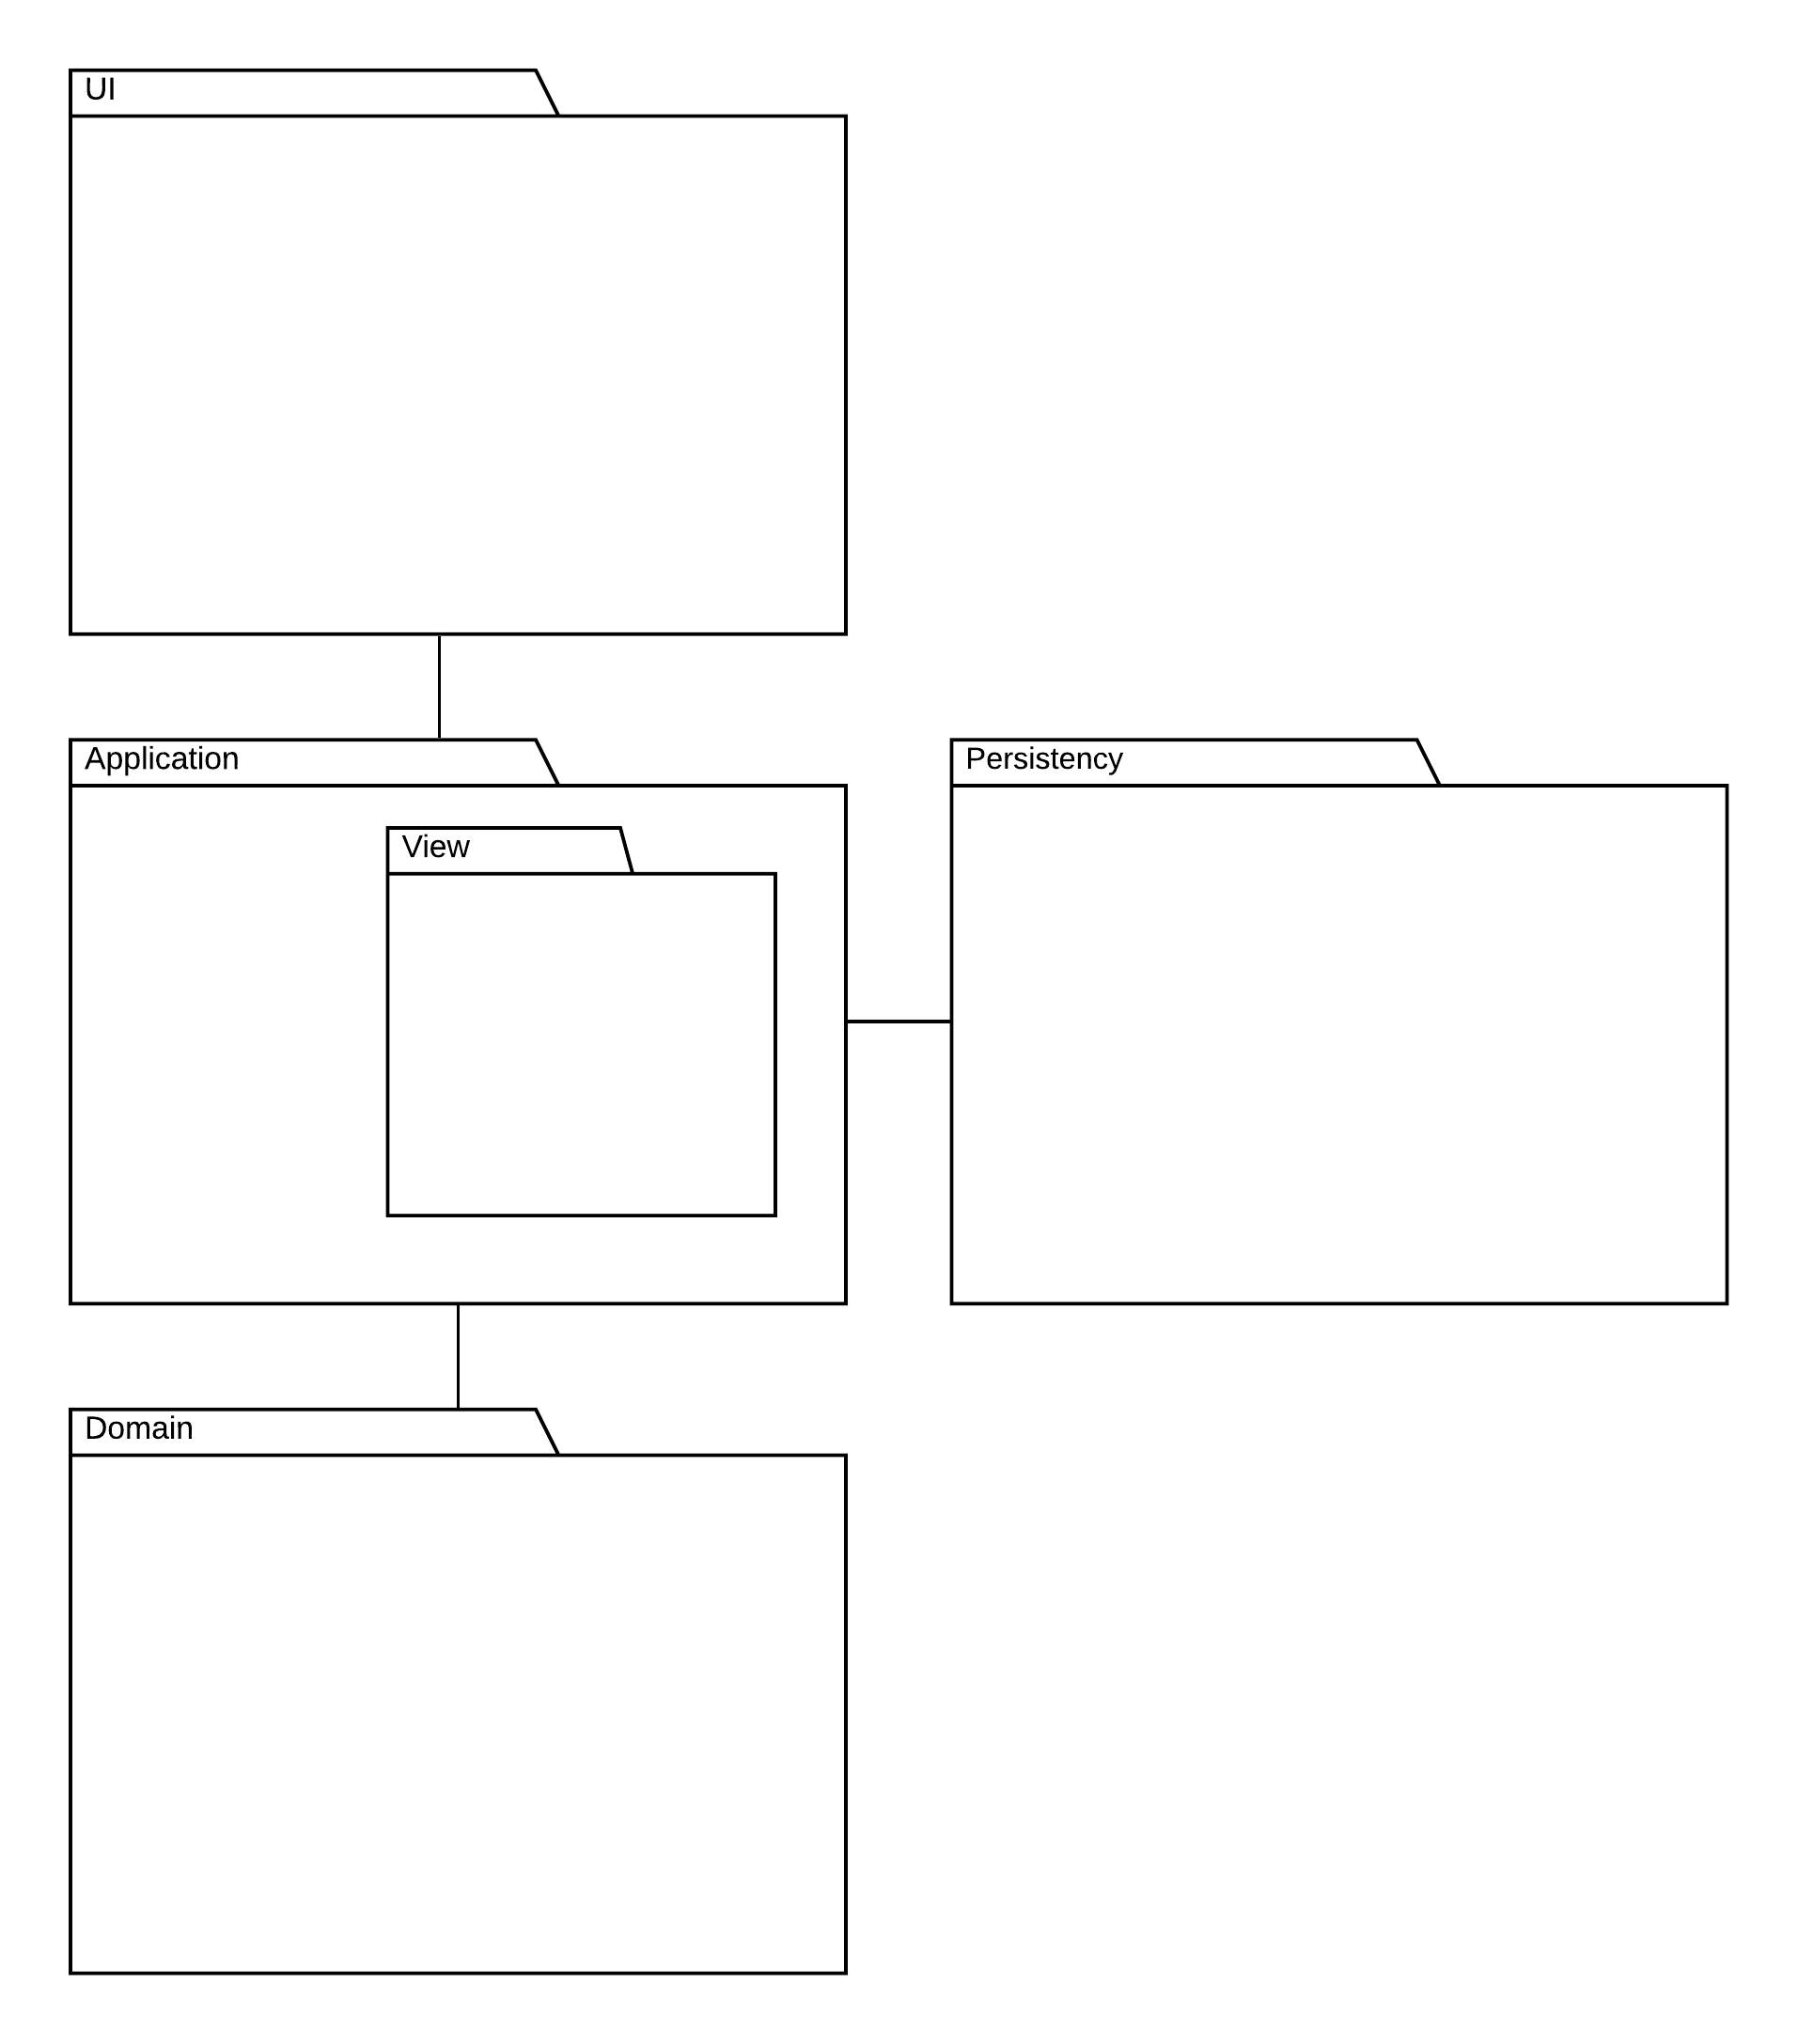
\includegraphics[width=\textwidth]{RelationDCD.png}
    \label{bilag:RelationDCD}
\end{figure}

\newpage
\begin{sidewaysfigure}[h]
    \caption{DCD for UI}
    \centering
        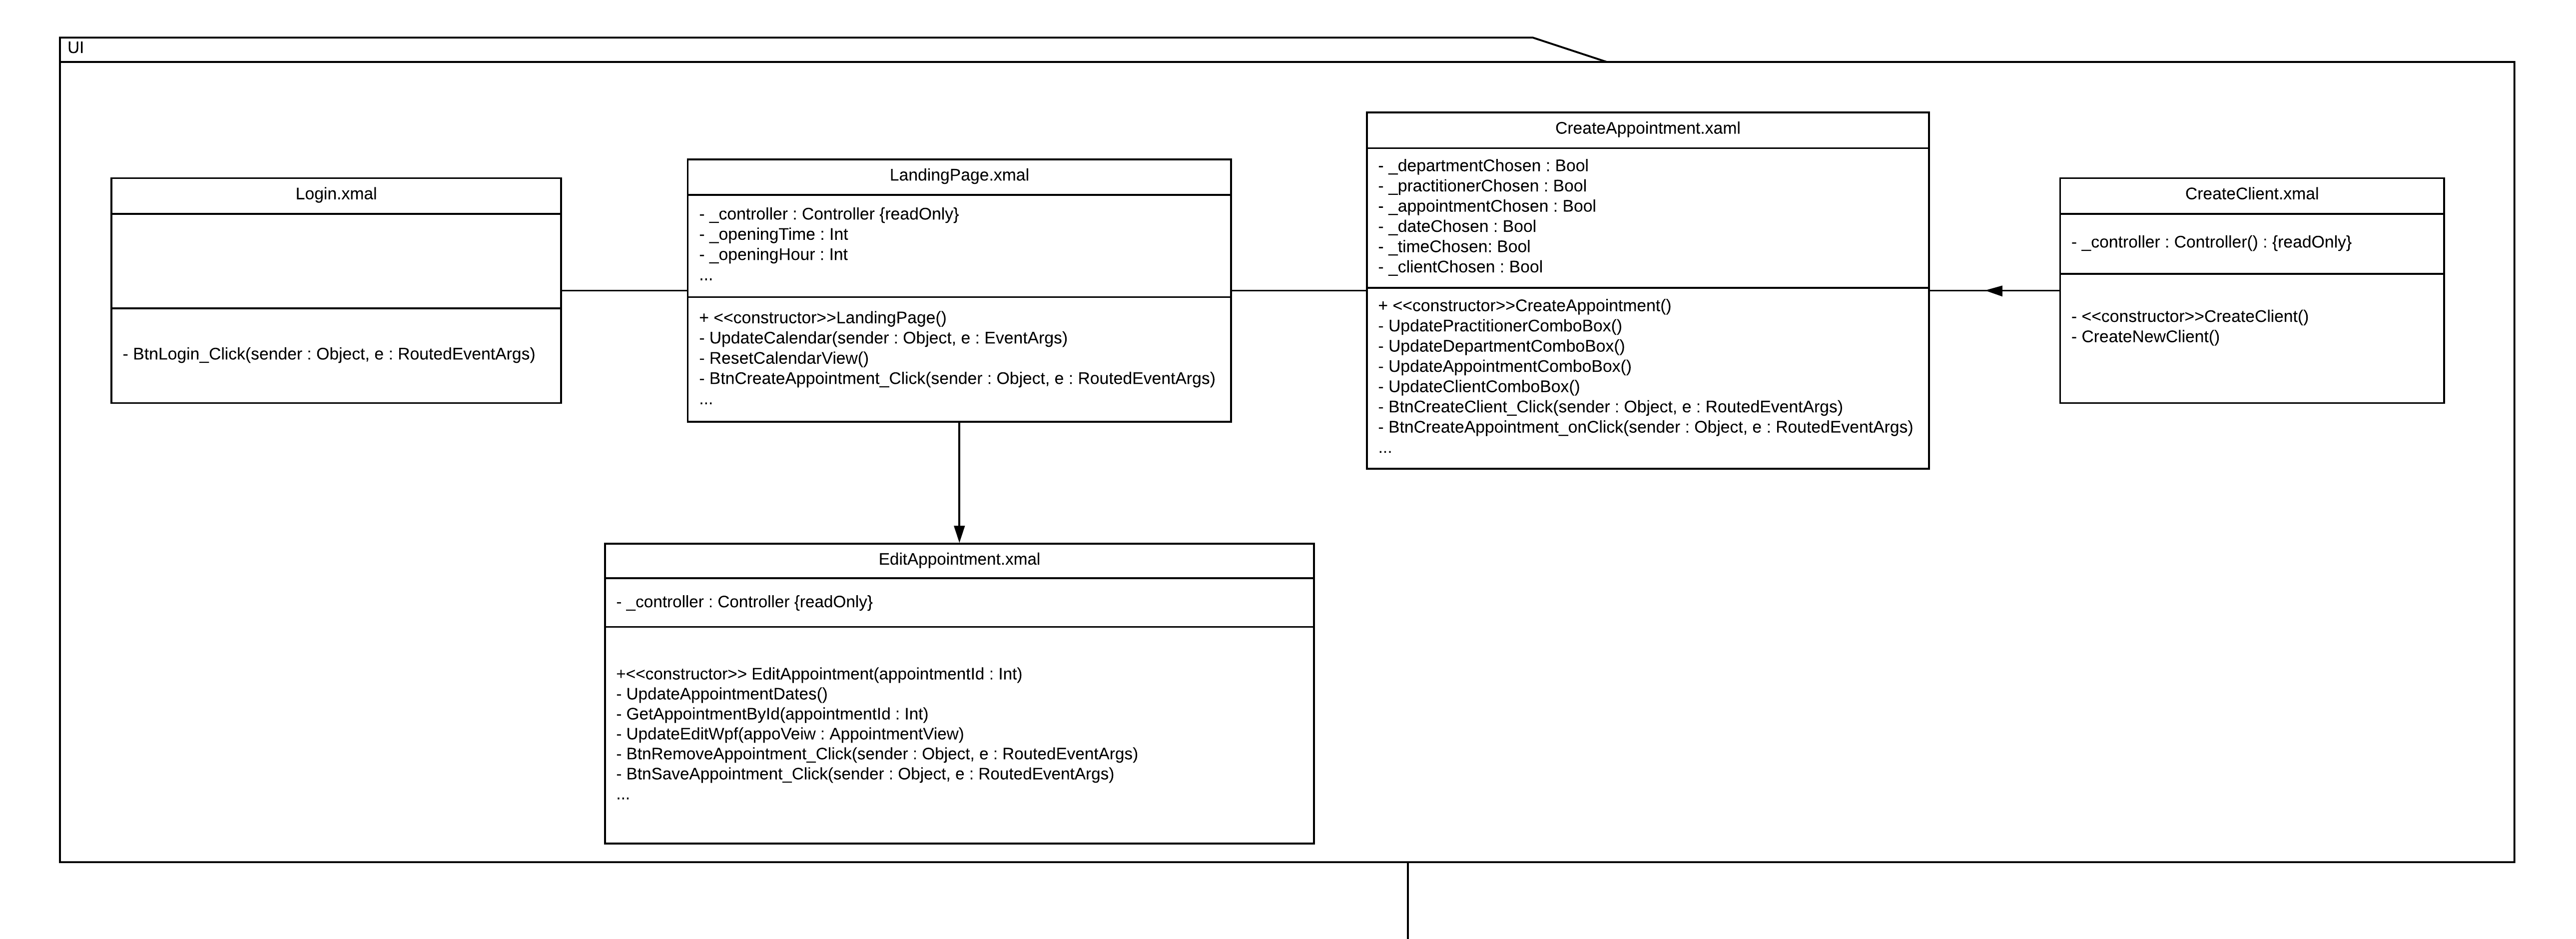
\includegraphics[width=\textwidth]{UIDCD.png}
    \label{bilag:UIDCD}
\end{sidewaysfigure}

\newpage
\begin{sidewaysfigure}[h]
    \caption{DCD for Application}
    \centering
        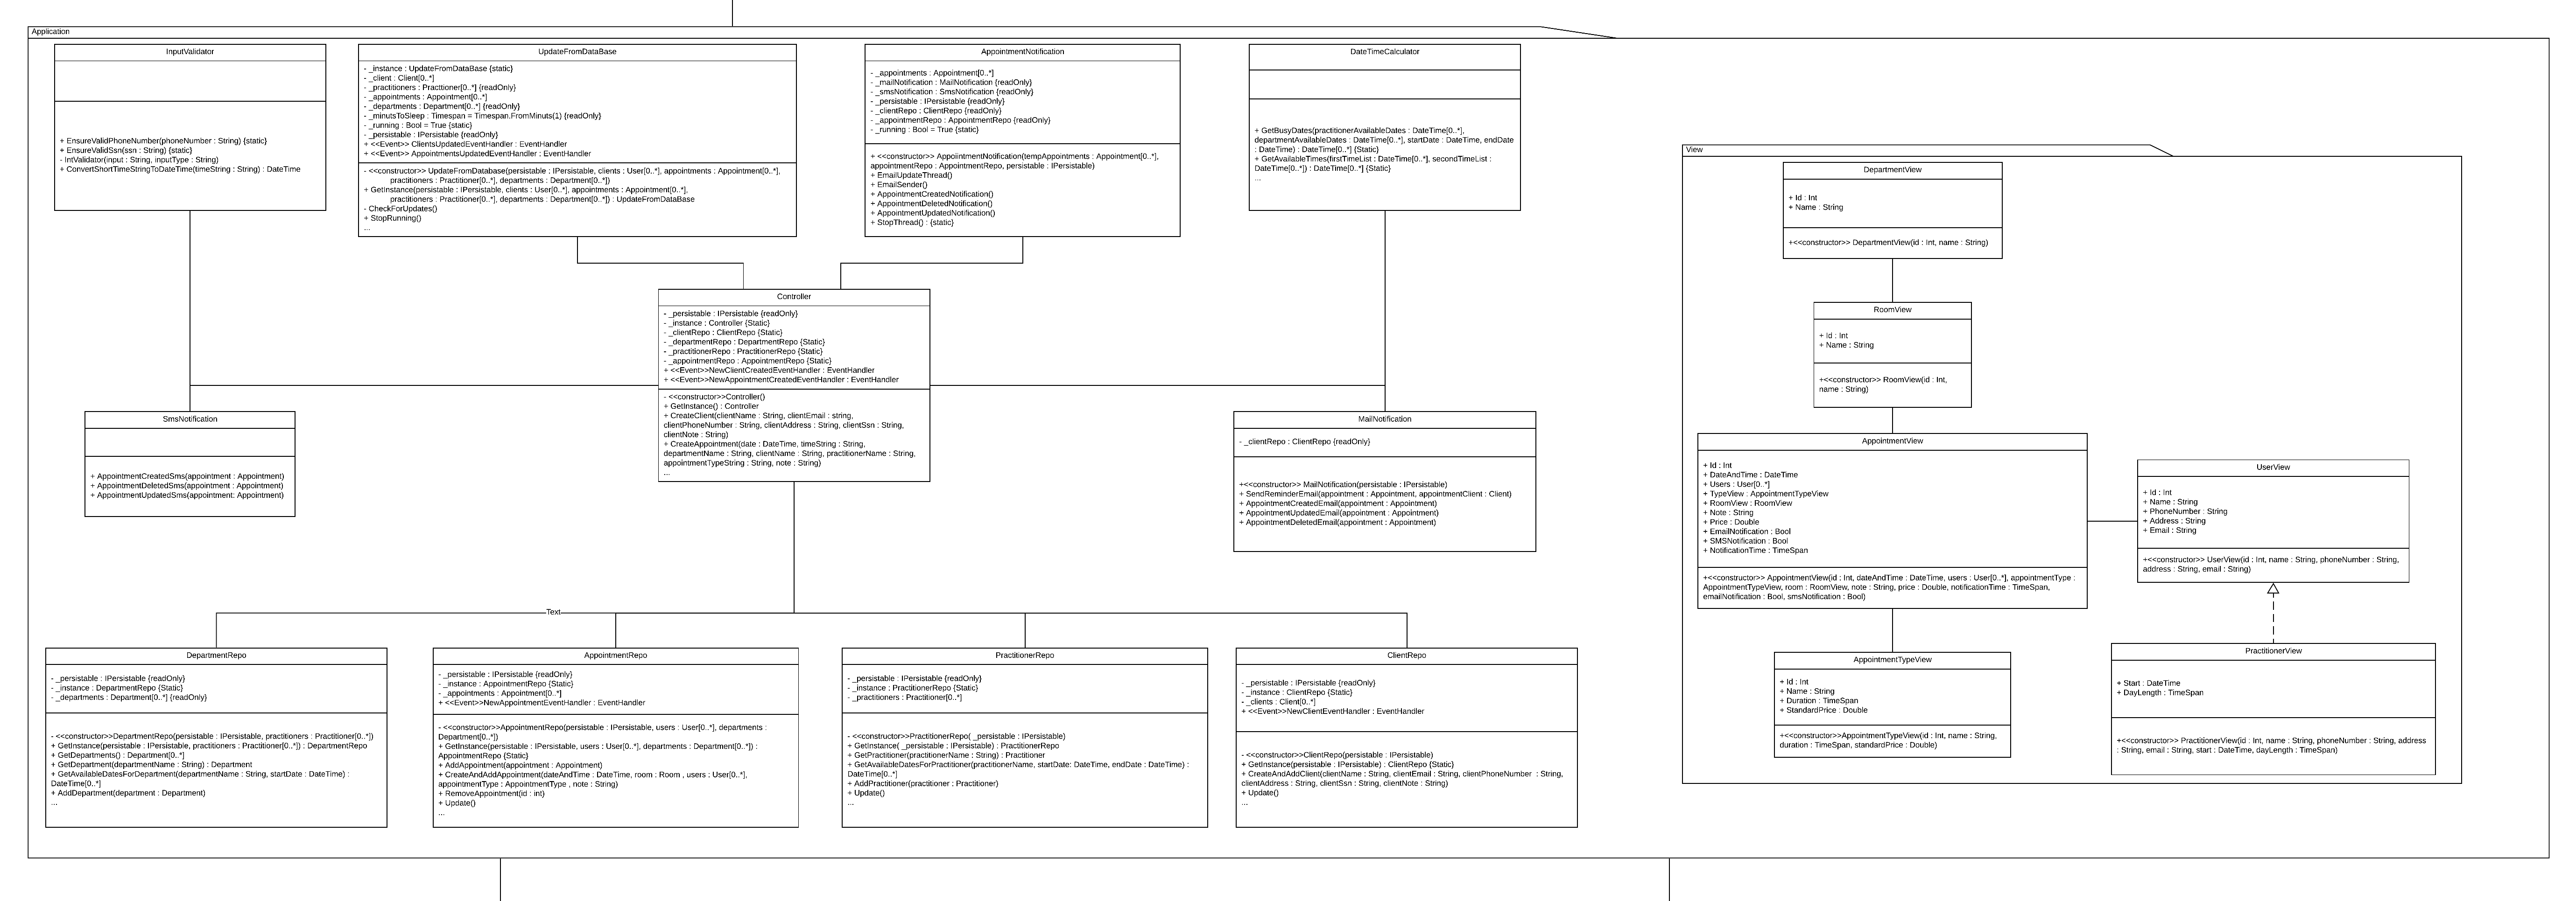
\includegraphics[width=\textwidth]{ApplicationDCD.png}
    \label{bilag:ApplicationDCD}
\end{sidewaysfigure}

\newpage
\begin{figure}[h]
    \caption{DCD for Domain}
    \centering
        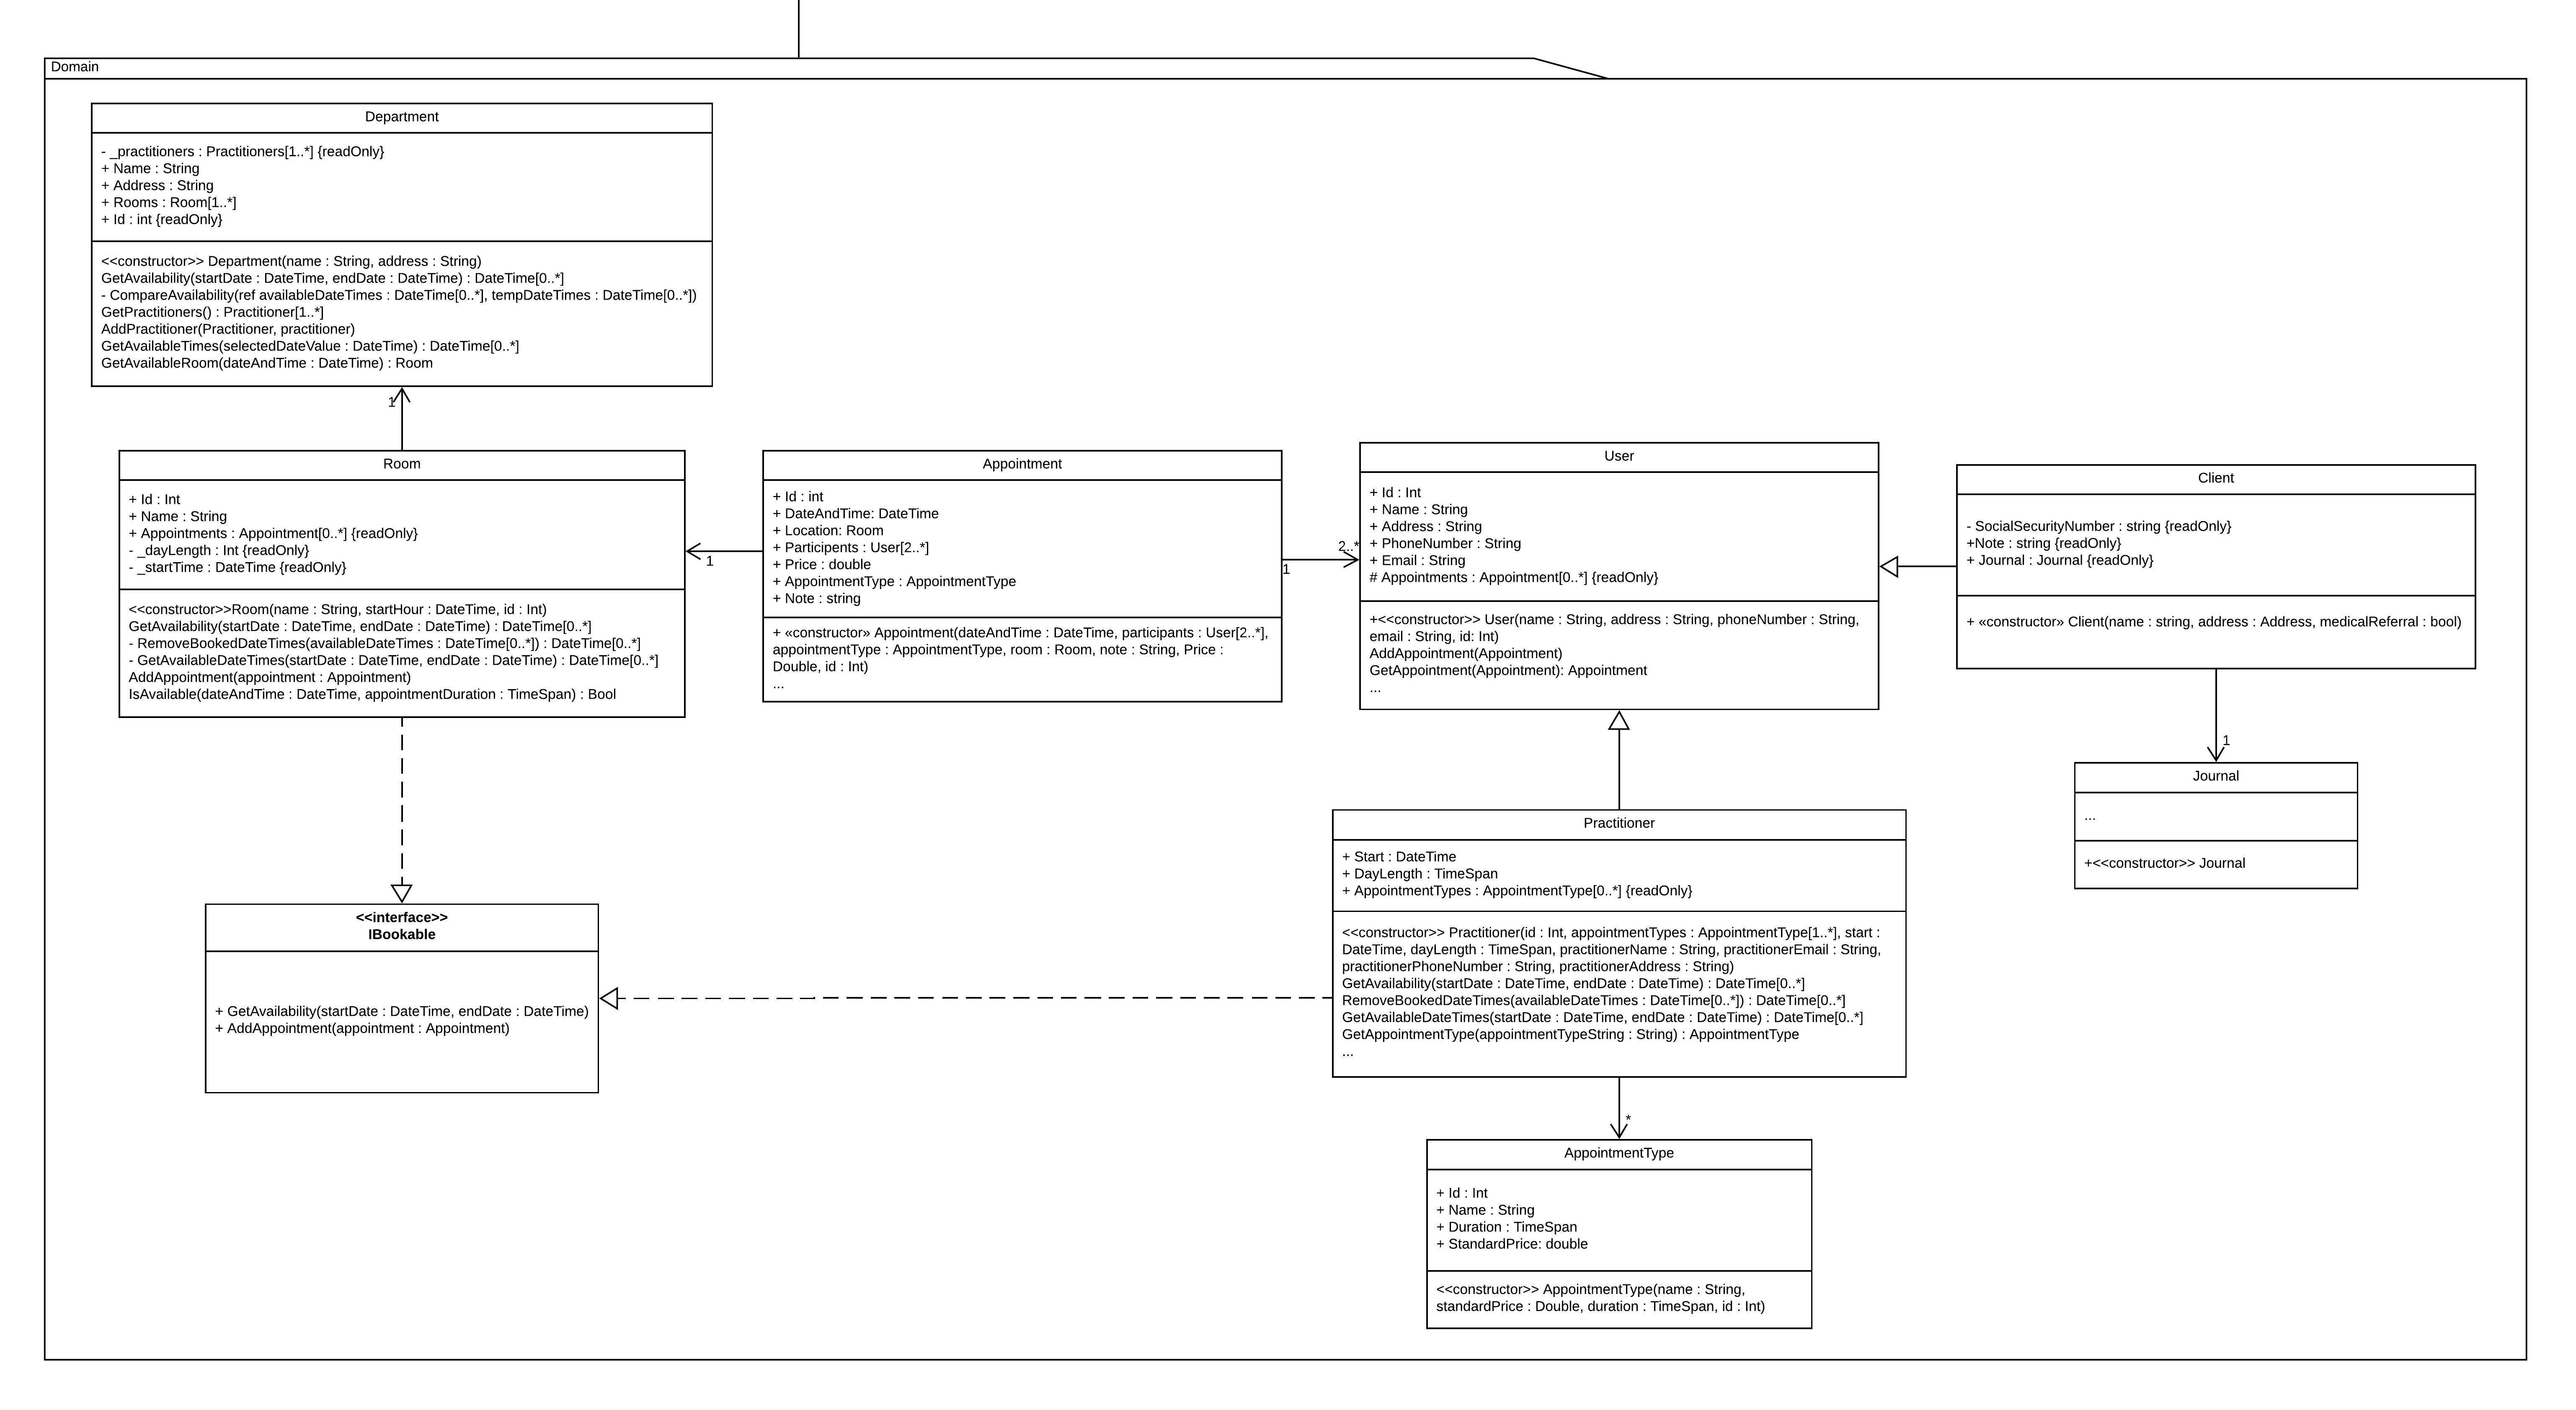
\includegraphics[width=\textwidth]{DomainDCD.png}
    \label{bilag:DomainDCD}
\end{figure}

\begin{figure}[h]
    \caption{DCD for Persistency}
    \centering
        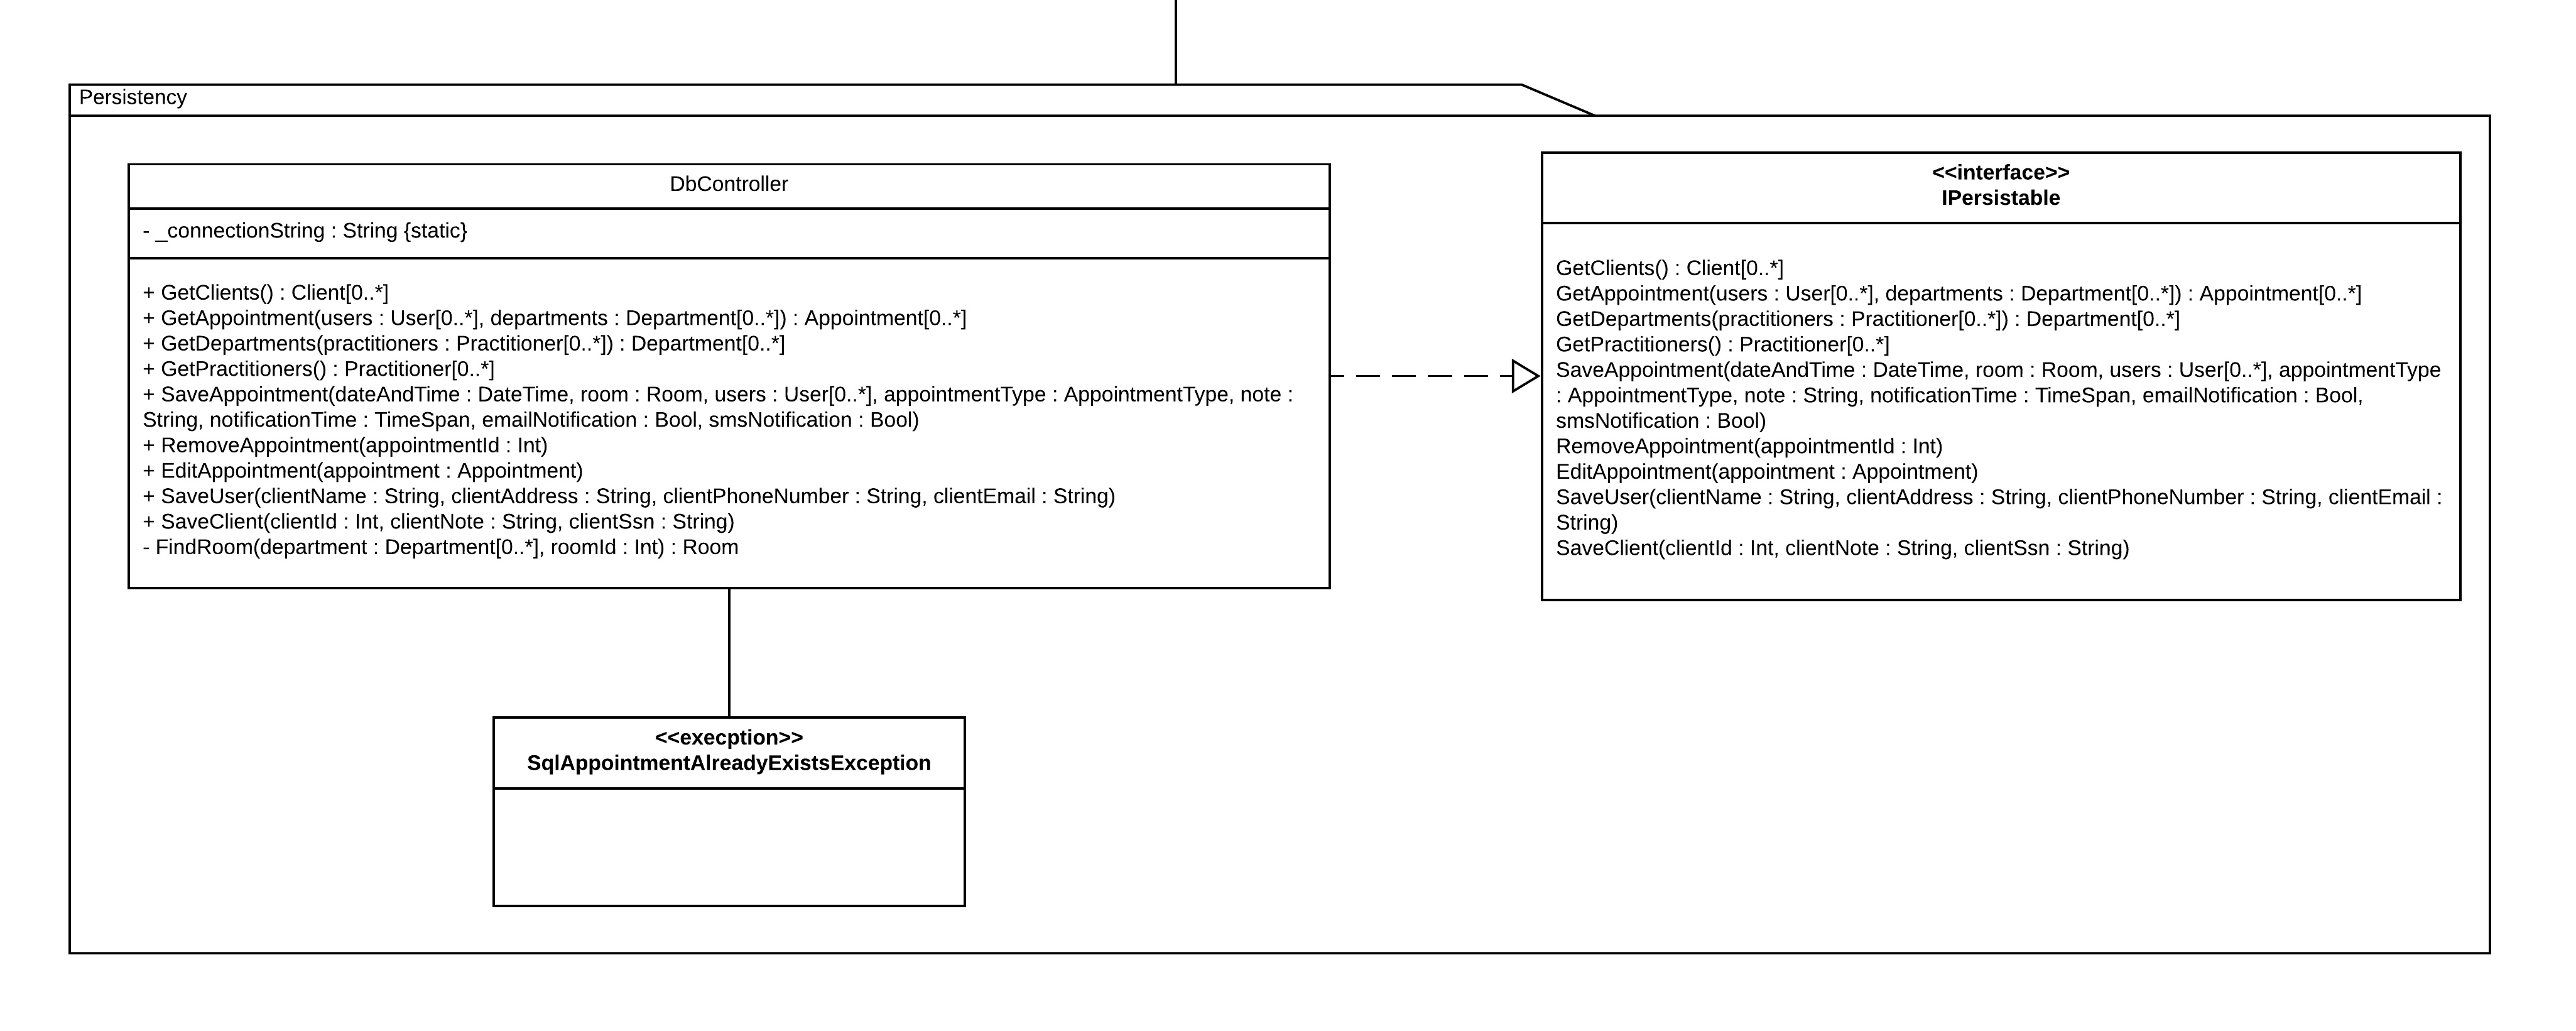
\includegraphics[width=\textwidth]{PersistableDCD.png}
    \label{bilag:PersistableDCD}
\end{figure}


\subsection{Kode}

\begin{figure}[h]
    \caption{Hjælpemetoder til CheckForUpdates metoden}
    \centering
        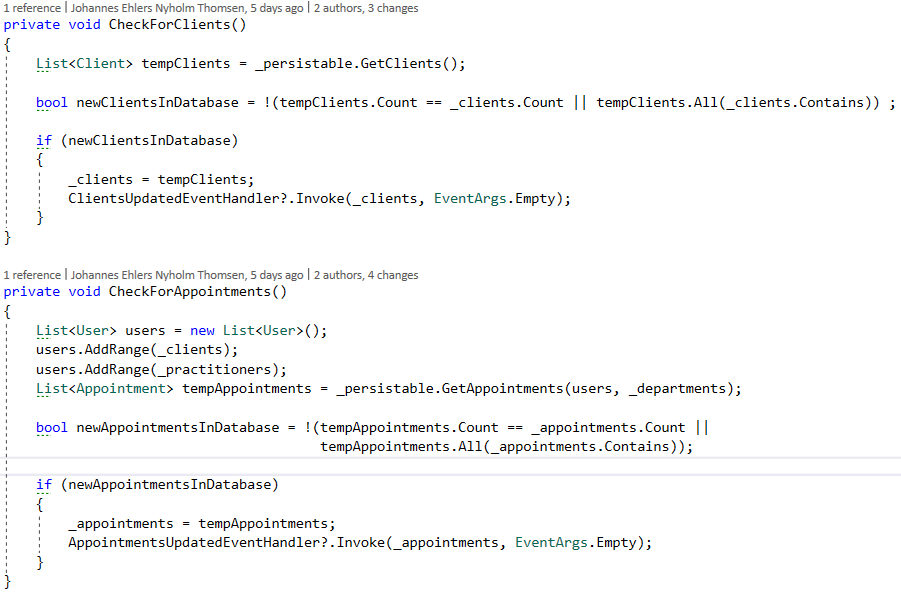
\includegraphics[width=\textwidth]{UpdateFromDatabaseHelpMethods.png}
    \label{bilag:CheckForUpdates }
\end{figure}